\documentclass{article}%
\usepackage[T1]{fontenc}%
\usepackage[utf8]{inputenc}%
\usepackage{lmodern}%
\usepackage{textcomp}%
\usepackage{lastpage}%
\usepackage[tmargin=1cm,bmargin=2cm,lmargin=1cm]{geometry}%
\usepackage{multicol}%
\usepackage{graphicx}%
\usepackage{adjustbox}%
\usepackage{tkz-euclide}%
\usepackage{amsmath}%
\usepackage{scalefnt}%
\usepackage{enumitem}%
%
%
%
\begin{document}%
\normalsize%
\setlength\itemsep{-2cm}%
\section{Graph a line given a point and its slope}%
\label{sec:Graphalinegivenapointanditsslope}%
\textbf{Learning Goal: }\hrulefill \\ \hrulefill%
\begin{multicols}{2}%
\begin{enumerate}[label=\arabic*),start=1]%
\item\adjustbox{valign=t}{\begin{minipage}{\linewidth}
Graph the line with y-intercept at $(0,4)$ and zero slope.\\

%\vspace{4cm}

\begin{tikzpicture}[font=\small,scale=0.40]
   \tikzstyle{every node}=[font=\small]
   \tkzInit[xmax=6,ymax=6,xmin=-6,ymin=-6]
   \tkzGrid
   \tkzAxeXY
%   \draw[ thick,latex-latex] (-1,4) -- (4,-6) node[anchor=south west] {$a$}; % two points for drawing 2x+y=2
%  \tkzText[above](0,6.75){Desired Output}
  \end{tikzpicture}
\end{minipage}}%
\vspace{0cm}%
\item\adjustbox{valign=t}{\begin{minipage}{\linewidth}
Graph the line through the origin with slope -$\frac{5}{2}$.\\

%\vspace{4cm}

\begin{tikzpicture}[font=\small,scale=0.40]
   \tikzstyle{every node}=[font=\small]
   \tkzInit[xmax=6,ymax=6,xmin=-6,ymin=-6]
   \tkzGrid
   \tkzAxeXY
%   \draw[ thick,latex-latex] (-1,4) -- (4,-6) node[anchor=south west] {$a$}; % two points for drawing 2x+y=2
%  \tkzText[above](0,6.75){Desired Output}
  \end{tikzpicture}
\end{minipage}}%
\vspace{0cm}%
\item\adjustbox{valign=t}{\begin{minipage}{\linewidth}
Graph the line through the origin with slope $\frac{1}{3}$.\\

%\vspace{4cm}

\begin{tikzpicture}[font=\small,scale=0.40]
   \tikzstyle{every node}=[font=\small]
   \tkzInit[xmax=6,ymax=6,xmin=-6,ymin=-6]
   \tkzGrid
   \tkzAxeXY
%   \draw[ thick,latex-latex] (-1,4) -- (4,-6) node[anchor=south west] {$a$}; % two points for drawing 2x+y=2
%  \tkzText[above](0,6.75){Desired Output}
  \end{tikzpicture}
\end{minipage}}%
\vspace{0cm}%
\item\adjustbox{valign=t}{\begin{minipage}{\linewidth}
Graph the line through the origin with slope $-2$.\\

%\vspace{4cm}

\begin{tikzpicture}[font=\small,scale=0.40]
   \tikzstyle{every node}=[font=\small]
   \tkzInit[xmax=6,ymax=6,xmin=-6,ymin=-6]
   \tkzGrid
   \tkzAxeXY
%   \draw[ thick,latex-latex] (-1,4) -- (4,-6) node[anchor=south west] {$a$}; % two points for drawing 2x+y=2
%  \tkzText[above](0,6.75){Desired Output}
  \end{tikzpicture}
\end{minipage}}%
\vspace{0cm}%
\item\adjustbox{valign=t}{\begin{minipage}{\linewidth}
Graph the line through the origin with slope $2$.\\

%\vspace{4cm}

\begin{tikzpicture}[font=\small,scale=0.40]
   \tikzstyle{every node}=[font=\small]
   \tkzInit[xmax=6,ymax=6,xmin=-6,ymin=-6]
   \tkzGrid
   \tkzAxeXY
%   \draw[ thick,latex-latex] (-1,4) -- (4,-6) node[anchor=south west] {$a$}; % two points for drawing 2x+y=2
%  \tkzText[above](0,6.75){Desired Output}
  \end{tikzpicture}
\end{minipage}}%
\vspace{0cm}%
\item\adjustbox{valign=t}{\begin{minipage}{\linewidth}
Graph the line with y-intercept (0,-2) and slope $3$.\\

%\vspace{4cm}

\begin{tikzpicture}[font=\small,scale=0.40]
   \tikzstyle{every node}=[font=\small]
   \tkzInit[xmax=6,ymax=6,xmin=-6,ymin=-6]
   \tkzGrid
   \tkzAxeXY
%   \draw[ thick,latex-latex] (-1,4) -- (4,-6) node[anchor=south west] {$a$}; % two points for drawing 2x+y=2
%  \tkzText[above](0,6.75){Desired Output}
  \end{tikzpicture}
\end{minipage}}%
\vspace{0cm}%
\item\adjustbox{valign=t}{\begin{minipage}{\linewidth}
Graph the line with y-intercept (0,4) and slope $0$.\\

%\vspace{4cm}

\begin{tikzpicture}[font=\small,scale=0.40]
   \tikzstyle{every node}=[font=\small]
   \tkzInit[xmax=6,ymax=6,xmin=-6,ymin=-6]
   \tkzGrid
   \tkzAxeXY
%   \draw[ thick,latex-latex] (-1,4) -- (4,-6) node[anchor=south west] {$a$}; % two points for drawing 2x+y=2
%  \tkzText[above](0,6.75){Desired Output}
  \end{tikzpicture}
\end{minipage}}%
\vspace{0cm}%
\item\adjustbox{valign=t}{\begin{minipage}{\linewidth}
Graph the line with x-intercept $(-4,0)$ and slope $\frac{3}{2}$.\\

%\vspace{4cm}

\begin{tikzpicture}[font=\small,scale=0.40]
   \tikzstyle{every node}=[font=\small]
   \tkzInit[xmax=6,ymax=6,xmin=-6,ymin=-6]
   \tkzGrid
   \tkzAxeXY
%   \draw[ thick,latex-latex] (-1,4) -- (4,-6) node[anchor=south west] {$a$}; % two points for drawing 2x+y=2
%  \tkzText[above](0,6.75){Desired Output}
  \end{tikzpicture}
\end{minipage}}%
\vspace{0cm}%
\item\adjustbox{valign=t}{\begin{minipage}{\linewidth}
Graph the line with x-intercept $(3,0)$ and slope $-1$.\\

%\vspace{4cm}

\begin{tikzpicture}[font=\small,scale=0.40]
   \tikzstyle{every node}=[font=\small]
   \tkzInit[xmax=6,ymax=6,xmin=-6,ymin=-6]
   \tkzGrid
   \tkzAxeXY
%   \draw[ thick,latex-latex] (-1,4) -- (4,-6) node[anchor=south west] {$a$}; % two points for drawing 2x+y=2
%  \tkzText[above](0,6.75){Desired Output}
  \end{tikzpicture}
\end{minipage}}%
\vspace{0cm}%
\item\adjustbox{valign=t}{\begin{minipage}{\linewidth}
Graph the line with x-intercept at $(-1,0)$ and y-intercept $(0,4)$.\\

%\vspace{4cm}

\begin{tikzpicture}[font=\small,scale=0.40]
   \tikzstyle{every node}=[font=\small]
   \tkzInit[xmax=6,ymax=6,xmin=-6,ymin=-6]
   \tkzGrid
   \tkzAxeXY
%   \draw[ thick,latex-latex] (-1,4) -- (4,-6) node[anchor=south west] {$a$}; % two points for drawing 2x+y=2
%  \tkzText[above](0,6.75){Desired Output}
  \end{tikzpicture}
\end{minipage}}%
\vspace{0cm}%
\item\adjustbox{valign=t}{\begin{minipage}{\linewidth}
Graph the line with y-intercept at $(-1,0)$ and x-intercept $(-5,0)$.\\

%\vspace{4cm}

\begin{tikzpicture}[font=\small,scale=0.40]
   \tikzstyle{every node}=[font=\small]
   \tkzInit[xmax=6,ymax=6,xmin=-6,ymin=-6]
   \tkzGrid
   \tkzAxeXY
%   \draw[ thick,latex-latex] (-1,4) -- (4,-6) node[anchor=south west] {$a$}; % two points for drawing 2x+y=2
%  \tkzText[above](0,6.75){Desired Output}
  \end{tikzpicture}
\end{minipage}}%
\vspace{0cm}%
\item\adjustbox{valign=t}{\begin{minipage}{\linewidth}
\\

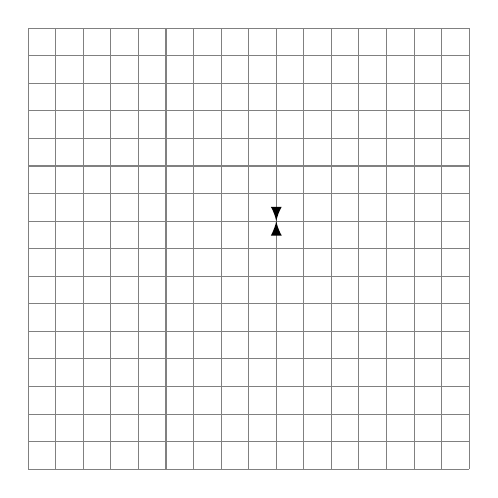
\begin{tikzpicture}[font=\tiny,scale=0.35]
   %\tikzstyle{every node}=[font=\small]
   \tkzInit[xmax=8,ymax=8,xmin=-8,ymin=-8]
   \tkzGrid
   \tkzAxeXY
   \draw[ thick,latex-latex] (,) -- (,);% node[anchor=south west] {$a$}; % two points for drawing 2x+y=2
%  \tkzText[above](0,6.75){Desired Output}
  \end{tikzpicture}
\end{minipage}}%
\vspace{0cm}%
\end{enumerate}

%
\end{multicols}%
\end{document}